%\subsection{Practical aspects}
%%%%%%%%%%%%%%%%%%%%%%%%%%%%%%%%%%%%%%%%%%%%%%%%%%%%%%%%%%%%%%%%%%%%%%
%\begin{frame}{Remarks on Plausibility of Assumptions}
%Assumption for theoretical analysis:
%\begin{itemize}
%	\item A1: Agents are modeled as double integrators
%	\item A2: The scalar field is assumed to be convex and twice differentiable
%	\item A3: Measurements of $\psi(q_i)$, $\nabla \psi(q_i)$ and $\nabla^2\psi(q_i)$ by agent $i$
%\end{itemize}
%\end{frame}
%%%%%%%%%%%%%%%%%%%%%%%%%%%%%%%%%%%%%%%%%%%%%%%%%%%%%%%%%%%%%%%%%%%%%
\begin{frame}{Towards Experiments: Modeling agents as double integrators}
\begin{figure}[h!]
	\tikzstyle{block} = [draw, rectangle, 
    minimum height=3em, minimum width=6em]
\tikzstyle{sum} = [draw,  circle, node distance=1cm]
\tikzstyle{input} = [coordinate]
\tikzstyle{output} = [coordinate]
\tikzstyle{pinstyle} = [pin edge={to-,thin,black}]

% The block diagram code is probably more verbose than necessary
%\begin{tikzpicture}[auto, node distance=2cm,>=latex']
%    % We start by placing the blocks
%    \node [input, name=input] {};
%    \node [sum, right of=input] (sum) {};
%    \node [block, right of=sum] (controller) {Controller};
%    \node [block, right of=controller, pin={[pinstyle]above:Disturbances},
%            node distance=3cm] (system) {System};
%    % We draw an edge between the controller and system block to 
%    % calculate the coordinate u. We need it to place the measurement block. 
%    \draw [->] (controller) -- node[name=u] {$u$} (system);
%    \node [output, right of=system] (output) {};
%    \node [block, below of=u] (measurements) {Measurements};
%
%    % Once the nodes are placed, connecting them is easy. 
%    \draw [draw,->] (input) -- node {$r$} (sum);
%    \draw [->] (sum) -- node {$e$} (controller);
%    \draw [->] (system) -- node [name=y] {$y$}(output);
%    \draw [->] (y) |- (measurements);
%    \draw [->] (measurements) -| node[pos=0.99] {$-$} 
%        node [near end] {$y_m$} (sum);
%\end{tikzpicture}

\begin{tikzpicture}[auto, node distance=2cm,>=latex']
% We start by placing the blocks
\node [input, name=input] {};
\node [block, right of=input,pin={[pinstyle]above:$\Psi(q)$},node distance=2.5cm](Flockcontrol) {$u=-\nabla V-(\hat{L}+cI)p + f_{\gamma} $};
\node [block, right of=Flockcontrol,node distance=3cm,minimum height=1em,minimum width=2em](integrator) {$\frac{1}{s}$};
\node [block, right of=integrator,node distance=2cm,minimum height=2.5em,minimum width=3em](velocityloop) {$G_{\textnormal{vel}}$};
\node [output, right of=velocityloop,node distance=1cm](output) {};
\node [block, below of=integrator,node distance=2cm](network) {Network};
% Once the nodes are placed, connecting them is easy. 
\draw [draw,->] (input) -- node {} (Flockcontrol);
\draw [draw,->] (Flockcontrol) -- node {} (integrator);
\draw [draw,->] (integrator) -- node {$p_{\textnormal{des}}$} (velocityloop);
\draw [draw,->] (velocityloop) -- node[name=outmid] {$\begin{bmatrix}q\\p\end{bmatrix}$} (output);
\draw [->] (outmid) |- (network);
\draw [-] (network) -| (input);
\end{tikzpicture}
	\caption{Control Architecture}
	\label{fig:control_arch}	
\end{figure}
\begin{itemize}
	\item The flocking loop is runs at 20Hz 
	\item $G_{\textnormal{vel}}$: closed loop velocity tracking loop runs at 100Hz
	\item Initial tests show that the velocity controller is fast enough $\implies$ approximate $G_{\textnormal{vel}}$ by single integrator dynamics.
\end{itemize}
\end{frame}
%%%%%%%%%%%%%%%%%%%%%%%%%%%%%%%%%%%%%%%%%%%%%%%%%%%%%%%%%%%%%%%%%%%%%%
%\begin{frame}{Towards Experiments: Convexity and differentiability of field}
%
%\begin{itemize}
%    \item The actual fields in the scenarios of interest will most likely not be convex and perhaps not smooth enough
%    \item Non-differentiability: Fit a locally smooth approximation
%    \item Non-convexity: The result can then be seen as a local convergence result
%    \item Experimental tests include log-convex fields and fields with 2 minima to probe the applicability of the algorithm when the assumption is violated.
%\end{itemize}
%\end{frame}
%%%%%%%%%%%%%%%%%%%%%%%%%%%%%%%%%%%%%%%%%%%%%%%%%%%%%%%%%%%%%%%%%%%%%
\begin{frame}{Towards Experiments: $\psi(q_i)$, $\nabla \psi(q_i)$, $\nabla^2\psi(q_i)$}
\begin{figure}[h!]	
		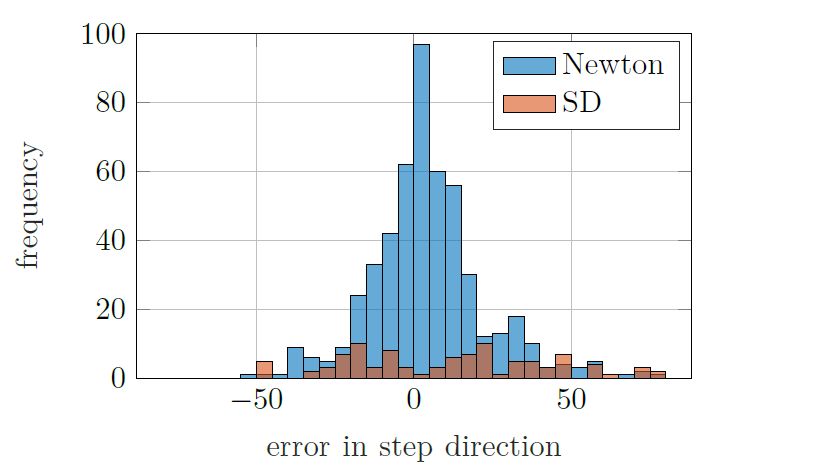
\includegraphics[width=7cm]{figures/newton_SD_direction.png}
		%\caption{Histograms of errors (in angles) between the estimated and true gradient direction and modified Newton step direction when the field measurements are corrupted}
		\label{fig:direction_errors_noise}
	\end{figure}
\begin{itemize}
	\item Corrupt the field strength measurement by +/- 5 percent of the field strength. 
	\item Estimate gradient by collecting local data and solving a least squares problem
	\item Estimate the hessian by collecting data from neighbors and solving another least squares problem
	\item Heuristic: Use Steepest Descent until the estimated hessian is positive definite.
\end{itemize}
\end{frame}